\chapter{Teori}\label{ch:Teroi}

I denne opgave er der brugt en række forskellige digitale filtre til at implementere en Audio equalizer. De forskellige filtre 
\begin{itemize}
\item FIR-filtre
\item IIR-filtre

\end{itemize}

\subsection{Equalizer}
En Equalizer er en , den .\\
Equaliseren er blevet implementeret ved at lave 5 forskellige båndpas filtre, der opdeler Audio-signalet i 5 forskellige frekvens dele. Disse båndpas filtre er blevet designet ved brug af IIR- og FIR-filtre. 
Der er et blokdiagram for Equalizeren på figur \ref{fig:Aktivitetsdiagram for Equalizeren}.

\begin{figure}[H]
	\centering
	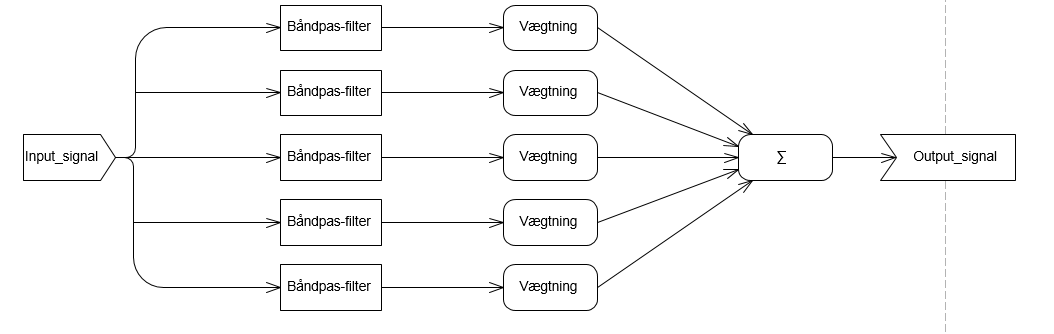
\includegraphics[width=150mm]{figures/Equalizer_flowchart.PNG}
	\caption{Aktivitetsdiagram for Audio Equalizeren}
	\label{fig:Aktivitetsdiagram for Equalizeren}
\end{figure}

I det nedenstående afsnit følger en beskrivelse af de to forskellige filtre type.
 
\subsection{FIR-filtre}
FIR står for Finite Implulse Response, hvilket betyder, at der er et endeligt antal af impulssvar.
Dette kan man se, i ligning \eqref{eq:FIR}, der er diffrensligningen for et FIR filter.
\begin{equation}\label{eq:FIR}
{y(n)} = \displaystyle\sum_{k=0}^{M-1} {b_{k}*x(n-k)}
\end{equation}


\subsection{IIR-filtre}
IIR står for Infinite Impulse Response, hvilket betyder, at det har et uendeligt antal output, da filteret benytter sig af feedback fra tidligere output. Hvis man kigger på ligning \eqref{eq:IIR} kan man se den generelle differensligning for et IIR-filter.



\begin{equation}\label{eq:IIR}
{y(n)} = \displaystyle\sum_{k=0}^{M-1} {b_{k}*x(n-k)}+\displaystyle\sum_{l=1}^{N-1} {a_{l}*y(n-l)}
\end{equation}

Man kan se den anvendte funktioner og en skabellon til et program i det vedhæftede bilag i afsnit \ref{ch:Bilag}.



